\documentclass[nooutcomes]{ximera}
%% handout
%% space
%% newpage
%% numbers
%% nooutcomes

%I added the commands here so that I would't have to keep looking them up
%\newcommand{\RR}{\mathbb R}
%\renewcommand{\d}{\,d}
%\newcommand{\dd}[2][]{\frac{d #1}{d #2}}
%\renewcommand{\l}{\ell}
%\newcommand{\ddx}{\frac{d}{dx}}
%\everymath{\displaystyle}
%\newcommand{\dfn}{\textbf}
%\newcommand{\eval}[1]{\bigg[ #1 \bigg]}

%\begin{image}
%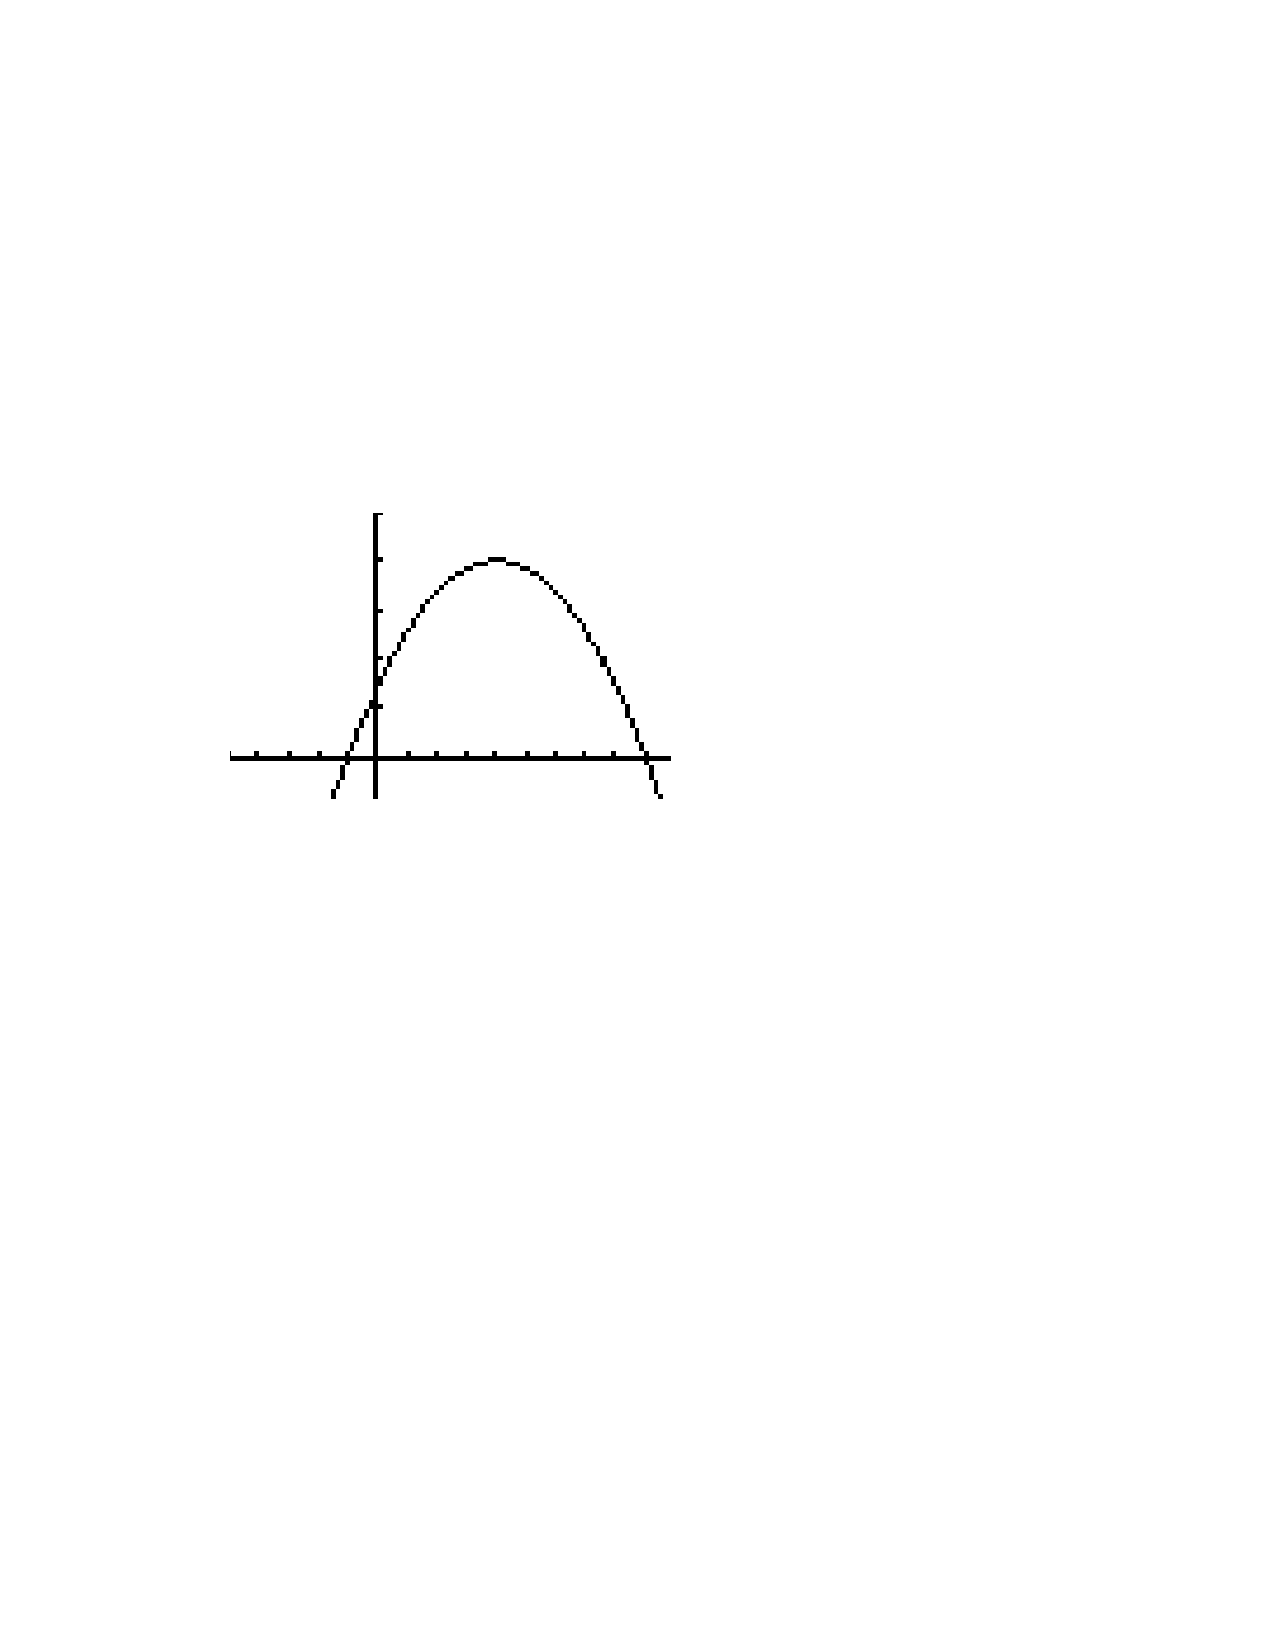
\includegraphics[trim= 170 420 250 180]{Figure1.pdf}
%\end{image}


\newcommand{\RR}{\mathbb R}
\renewcommand{\d}{\,d}
\newcommand{\dd}[2][]{\frac{d #1}{d #2}}
\renewcommand{\l}{\ell}
\newcommand{\ddx}{\frac{d}{dx}}
\newcommand{\dfn}{\textbf}
\newcommand{\eval}[1]{\bigg[ #1 \bigg]}

\usepackage{multicol}

\renewenvironment{freeResponse}{
\ifhandout\setbox0\vbox\bgroup\else
\begin{trivlist}\item[\hskip \labelsep\bfseries Solution:\hspace{2ex}]
\fi}
{\ifhandout\egroup\else
\end{trivlist}
\fi} %% we can turn off input when making a master document

\title{3.10: Derivatives of Inverse Trig Functions}  

\begin{document}
\begin{abstract}		\end{abstract}
\maketitle


%problem1
\begin{problem}
  A table of values for $f$ and $f'$ is shown below.
  Suppose that $f$ is a one-to-one function and $f^{-1}$ is its inverse.
  \begin{center}
    \begin{tabular}{ccc}
\hline
      $x$ & $f(x)$ & $f'(x)$\\
\hline \hline
      1 & 3 & 4\\

      3 & 4 & 5\\

      4 & 6 & 3\\
\hline
    \end{tabular}
  \end{center}

  \begin{enumerate}
    \item Evaluate $f^{-1}(f(x))$ at $x = 3$.
      \begin{freeResponse}
         $ f^{-1}(f(3)) = f^{-1}(4) = 3$
      \end{freeResponse}


    \item Evaluate $\ddx f(f(x))$ at $x = 3$.
      \begin{freeResponse}

        \begin{align*}
          \ddx f(f(x)) = f'(f(x)) \cdot f'(x) &\implies \eval{\ddx}_{x = 3} f(f(x)) = f'(f(3)) \cdot f'(3)\\
          &= f'(4) \cdot 5 = 3 \cdot 5 = 15
        \end{align*}
      \end{freeResponse}


    \item Evaluate $\ddx\ln((f(x))$ at $x = 3$.
      \begin{freeResponse}

        \begin{align*}
          \ddx\ln((f(x)) = \frac{f'(x)}{f(x)} \\
          &\implies \eval{\ddx \ln(f(x))}_{x = 3} = \frac{f'(3)}{f(3)} = \frac{5}{4}
        \end{align*}
      \end{freeResponse}


    \item Evaluate $f^{-1}(x)$ at $x = 3$.
      \begin{freeResponse}
	$ f^{-1}(3) = 1 \iff 3 = f(1)$
      \end{freeResponse}


    \item Evaluate $\ddx f^{-1}(x)$ at $x = 3$.
      \begin{freeResponse}
        \begin{align*}
          \ddx f^{-1}(x) &= \frac{1}{f'(f^{-1}(x))} \\
          &\implies \eval{\ddx f^{-1}(x)}_{x = 3} = \frac{1}{f'(f^{-1}(3))} \\
          &= \frac{1}{f'(1)} = \frac{1}{4}
        \end{align*}
      \end{freeResponse}
      
      \item Evaluate $\lim_{x \to 4} \frac{f(x)-f(4)}{x-4}$
      \begin{freeResponse}
$\lim_{x \to 4} \frac{f(x)-f(4)}{x-4} = f'(4)=3$
      \end{freeResponse}
  \end{enumerate}
\end{problem}


%problem2
\begin{problem}
Find the derivative of $f^{-1}$ at the following points without solving for $f^{-1}$.
	\begin{enumerate}
	
	\item  $f(x) = x^2 + 1$ (for $x \geq 0$) at the point $(5,2)$.  
		\begin{freeResponse}
		$(f^{-1})'(5) = \frac{1}{f'(2)}$.  Since $f'(x) = 2x$, $f'(2) = 4$.  Thus, $(f^{-1})'(5) = \frac{1}{4}$.  
		\end{freeResponse}

	\item  $f(x) = x^2 - 2x - 3$ (for $x \leq 1$) at the point $(12, -3)$.  
		\begin{freeResponse}
		$(f^{-1})'(12) = \frac{1}{f'(-3)}$.  Since $f'(x) = 2x - 2$, $f'(-3) = -6 - 2 = -8$.  Thus, $(f^{-1})'(12) = - \frac{1}{8}$. 
		\end{freeResponse}
	\end{enumerate}
\end{problem}


%problem3
\begin{problem}
  \outcome{Find derivatives of inverse functions in general.}
  \outcome{Understand how the derivative of an inverse function relates to the original derivative.}
  Find the slope of the tangent line to the curve $y = f^{-1}(x)$ at $(4,7)$ if the slope of the tangent line to the curve $y=f(x)$ at $(7,4)$ is $\frac{2}{3}$.
  \begin{freeResponse}
    Note that the statement ``the slope of the tangent line to the curve $y=f(x)$ at $(7,4)$ is $\frac{2}{3}$" specifically means that $f'(7) = \frac{2}{3}$.
    The slope of the tangent line to the curve $y = f^{-1}(x)$ at $(4,7)$ is $(f^{-1})'(4)$, and so we use the formula for the derivative of the inverse function to compute: $(f^{-1})'(4) = \frac{1}{f'(7)} = \frac{1}{\frac{2}{3}} = \frac{3}{2}$.
  \end{freeResponse}
\end{problem}





\end{document} 


















